\documentclass[aps, 12pt]{revtex4}
\usepackage[english]{babel}
\usepackage[utf8]{inputenc}
\usepackage[T1]{fontenc}
% \usepackage{NotesTeX}
\usepackage{subfigure}
\usepackage{tikz}
\usetikzlibrary{arrows}
\usepackage{multirow}
\usepackage{listings}
\usepackage{extarrows}
\usepackage{parskip}
\usepackage{eurosym}
\usepackage{footmisc}
\usepackage{kantlipsum}
\usepackage{algorithm}
\usepackage{algpseudocode}


\def\thesection{\arabic{section}}
\def\thesubsection{\arabic{subsection}}
% \def\thesection{\arabic{section}}
\setcounter{secnumdepth}{4}


\renewcommand{\deg}{^{\circ}}
\newcommand\numberthis{\addtocounter{equation}{1}\tag{\theequation}}
\newcommand{\hksqrt}[2][]{\ \mathpalette\DHLhksqrt{[#1]{#2\,}}}
\def\DHLhksqrt#1#2{\setbox0=\hbox{$#1\sqrt#2$}\dimen0=\ht0
    \advance\dimen0-0.3\ht0
    \setbox2=\hbox{\vrule height\ht0 depth -\dimen0}
    {\box0\lower0.65pt\box2}}

\graphicspath{{figs/}}
\newcommand{\includegraphicsmaybe}[2][]{\IfFileExists{../plots/#2}{\includegraphics[#1]{#2}}{\includegraphics[width=0.7\linewidth]{giffel.jpg}}}



\begin{document}

\author{Håkon Olav Torvik}
\title{\Huge Problem Set 5 \\ \small Math228B Numerical solutions to differential equations}
\affiliation{UC Berkeley}
\date{\today}


\maketitle

\section*{Time-harmonic Waveguide Simulations}

I will solve a 2D Helmholtz problem for a given wavenumber $k$ with Sommerfeld radiation conditions at the boundaries.

\subsection{Method}


The specific boundary-value problem is formulated as
\begin{align}
    -\nabla^2u-k^2u               & = 0   &  & \text{in}\hspace{2mm} \Omega, \label{eq:pde}
    \\
    \mathbf{n}\cdot\nabla u       & = 0   &  & \text{on}\hspace{2mm} \Gamma_{\text{wall}},\label{eq:bwall}
    \\
    \mathbf{n}\cdot\nabla u + iku & = 0   &  & \text{on}\hspace{2mm} \Gamma_{\text{out}}, \label{eq:bout}
    \\
    \mathbf{n}\cdot\nabla u + iku & = 2ik &  & \text{on}\hspace{2mm} \Gamma_{\text{in}}. \label{eq:bin}
\end{align}

\subsubsection{Galerkin formulation}
Finding the weak-form of the bvp, I multiply \eqref{eq:pde} with a weight-function $v$ and integrate, obtaining

\begin{align}\label{eq:weak}
    \int_{\Omega} -\nabla^2u vdx - \int_{\Omega}k^2uvdx = 0.
\end{align}

Applying the divergence theorem on the first term yields
\begin{align*}
    \int_{\Omega}\nabla^2uvdx = \int_{\Omega}\nabla u\nabla vdx - \oint_{\Gamma}gvds,
\end{align*}

where $g = g_{\Gamma} = \mathbf{n}\cdot \nabla u\big |_{\Gamma}$ is the solution at the boundary. As the boundary $\Gamma$ is composed of sections, the last term can be split in three, and I obtain

\begin{align*}
    \oint_{\Gamma}gvds = & \int_{\Gamma_{\text{wall}}}g_{\text{wall}}vds + \int_{\Gamma_{\text{out}}}g_{\text{out}}vds + \int_{\Gamma_{\text{int}}}g_{\text{int}}vds
    \\
    =                    & \int_{\Gamma_{\text{wall}}}0\cdot vds + \int_{\Gamma_{\text{out}}}-ikuvds + \int_{\Gamma_{\text{int}}}(2ik-iku)vds
\end{align*}

Putting this all back into \eqref{eq:weak}, gives the final formulation

\begin{align}\label{eq:weak_galerkin}
    \int_{\Omega}\nabla u\nabla vdx-k^2\int_{\Omega}uvdx+ik\left(\int_{\Gamma_{\text{out}}}uvds+\int_{\Gamma_{\text{in}}}uvds \right) = 2ik\int_{\Gamma_{\text{in}}}vds,
\end{align}

where the Galerkin formulation is obtained by insiting that the weight-function $v$ is from the same function space as the solution $u$. This function space $V_h$ is the set of continous piece-wise linear functions on the domin $\Omega$ described by the mesh $T_h$, as such
\begin{equation}\label{eq:fnspace}
    V_h = \{v\in C^0(\Omega):v|_K\in \mathcal{P}_1(K)\forall K\in T_h  \}
\end{equation}

\subsubsection{Discretising}
Choosing a basis $\{\varphi_i = \varphi(K_i)\}$ for $V_h$, such that $\varphi_j\varphi_i=\delta_{ij} \forall K\in T_h$. The solution $u$ is expressed as a linear combination of these as $u=\sum_ju_j\varphi_j$.

In this basis, \eqref{eq:weak_galerkin} becomes the $n$ coupled equations, indexed with $i$
\begin{align*}
    \sum_ju_j\left[ \int_{\Omega}\nabla \varphi_j\nabla\varphi_idx-k^2\int_{\Omega}\varphi_j\varphi_ids + ik\left(\int_{\Gamma_{\text{in}}}\varphi_j\varphi_jds+\int_{\Gamma_{\text{out}}}\varphi_j\varphi_jds\right) \right] & \\ =2ik\int_{\Gamma_{\text{in}}}\varphi_ids&,
    \hspace{4mm}i=1,\dots n.
\end{align*}

This can be written much simpler as $A\mathbf{u}=\mathbf{b}$, where
\begin{align*}
    A                     & = K - k^2M + ik\left(B_{\text{in}}+B_{\text{out}}\right)
    \\
    K_{ij}                & = \int_{\Omega}\nabla \varphi_j\nabla\varphi_idx \numberthis{} \label{eq:mat_K}
    \\
    M_{ij}                & = \int_{\Omega}\varphi_j\varphi_idx  \label{eq:mat_M} \numberthis{}
    \\
    B_{\text{in/out}, ij} & = \int_{\Gamma_{\text{in/out}}}\varphi_j\varphi_ids  \label{eq:mat_B} \numberthis{}
    \\
    \mathbf{b}            & = 2ik\mathbf{b}_{\text{in}}
    \\
    b_{\text{in}, i}      & = \int_{\Gamma_{\text{in}}}\varphi_ids  \label{eq:mat_b} \numberthis{}
\end{align*}

\subsubsection{Transmitted intensity}
The transmitted intensity $H$ measured at the output boundary is, given a solution $u$, defined as
\begin{equation*}
    H(u) = \int_{\Gamma_{\text{out}}}|u|^2ds.
\end{equation*}

Numerically, this can be found as

\begin{align*}
    \int_{\Gamma_{\text{out}}}|u|^2ds & = \int_{\Gamma_{\text{out}}}u^*uds
    \\ &= \int_{\Gamma_{\text{out}}} \sum_ju_j^*\varphi_j\sum_iu_i\varphi_ids
    \\
                                      & = \sum_{ij}u_j^*u_i\int_{\Gamma_{\text{out}}}\varphi_j\varphi_ids
    \\ &= \sum_{ij}u_j^*B_{\text{out}, ij}u_i
    \\ &= \mathbf{u}^HB_{\text{out}}\mathbf{u}
\end{align*}

The intensity is a measure of how much of the energy of the wave from the input bounadry reaches the output boundary, and takes a value between 0 and 1.


\subsection{Verification}
Before applying the method on a real problem, I test it on a simple domain with an analytical solution.

\subsubsection{Exact solution}
The specific boundaries of the rectangular verification domain is given in the problem description. The exact solution is $u_e=e^{-ikx}$. Showing this by inserting into \eqref{eq:pde}-\eqref{eq:bin}. Using normal vectors $\mathbf{n}$ pointing out of domain $\Omega$.

\begin{align*}
    \nabla u_e =                   & \begin{pmatrix}
        \partial_x \\
        \partial_y
    \end{pmatrix} u_e = \begin{pmatrix}
        -ik \\ 0
    \end{pmatrix} u_e
    \\
    \nabla^2u_e =                  & \partial_x^2u_e + \partial_y^2u_e = (-ik)^2 u = -k^2u_e
    \\
    \\
    \eqref{eq:pde}: \hspace{2mm}   & -\nabla^2u_e-k^2u_e = k^2u_e - k^2u_e = 0
    \\
    \eqref{eq:bwall}: \hspace{2mm} & \mathbf{n}_{\text{wall}} = \begin{pmatrix}
        0 \\ \pm 1
    \end{pmatrix} \rightarrow \mathbf{n}\cdot \nabla u = \begin{pmatrix}
        0 \\ \pm
    \end{pmatrix}\cdot \begin{pmatrix}
        -ik \\ 0
    \end{pmatrix}u_e = 0
    \\
    \eqref{eq:bout}: \hspace{2mm}  & \mathbf{n}_{\text{out}} = \begin{pmatrix}
        1 \\ 0
    \end{pmatrix} \rightarrow \mathbf{n}\cdot \nabla u_e + iku = -iku_e + iku_e = 0
    \\
    \eqref{eq:bin}: \hspace{2mm}   & \mathbf{n}_{\text{in}} = \begin{pmatrix}
        -1 \\ 0
    \end{pmatrix} \rightarrow \mathbf{n}\cdot \nabla u_e + iku = iku_e + iku_e = 2iku_e
\end{align*}
For boundary condition at the input boundary, I use the fact that $x_{in}= 0$, such that $2iku_e(x_{in})= 2ik$. Thus, the exact solution does indeed satisfy the differential equation itself, and all the boundary conditions. Note that this solution is exact for all rectangular boundaries, though a translation is needed if $x_{in}\neq 0$.

\subsubsection{Boundaries}
I write a function \begin{verbatim}
    ein, eout, ewall = waveguide_edges(p, t)
\end{verbatim} that determines the input and output boundaries of a mesh (p, t).

\subsubsection{Computing matrices}
Using the stamping method, I write a function \begin{verbatim}
    K, M, Bin, Bout, bin = femhelmholtz(p, t, ein, eout)
\end{verbatim}
that stamps \texttt{sK}, \texttt{sM}, \texttt{sBin}, \texttt{sBout} and \texttt{sbin} into the right place in \texttt{K}, \texttt{M}, \texttt{Bin}, \texttt{Bout}, \texttt{bin}.

On an element $T_k$, the basis function are $\varphi_i=a_i+b_ix+c_iy$. $K_{ij}$, \eqref{eq:mat_K}, is given by the same expression as $A_{ij}$ from PS4, and in general given by \begin{equation*}
    sK_{ij} = \text{area}(T_k)(b_ib_j + c_ic_j).
\end{equation*}

I derive the value of the element matrix $sM$ in Appendix  \ref{apx:M}. It is in general given by
\begin{equation*}
    sM = \text{area}(T_k)\frac{1}{12}
    \begin{pmatrix}
        2 & 1 & 1 \\ 1 & 2 & 1 \\ 1 & 1 & 2
    \end{pmatrix}.
\end{equation*}

There are 3 non-zero basis function on each element. Along the boundary edges there are only two, $f(x) = 1-\frac{x}{x_1}$, and $g(x)=\frac{x}{x_1}$, where one of the sides of the element is placed at $x=0$. The element matrices at the boundaries are then
\begin{equation*}
    sB_{\text{in/out}} = \frac{d}{3}\begin{pmatrix}
        2 & 1 \\ 1 & 2
    \end{pmatrix},
\end{equation*}
where $d$ is the length of the boundary edge. Similarly, the element load is
\begin{equation*}
    sb_{\text{in}}=\frac{d}{2}\begin{pmatrix}
        1 \\ 1
    \end{pmatrix}.
\end{equation*}

\subsubsection{Testing method and determining convergence}
Solving the problem on the rectangular domain, and finding the error using the max-norm for several refinements of the mesh, I log-log-plot the error as function of element size, and determine the slope. This is shown in Figure \ref{fig:helmholtz_conv}. The slope is close to 2, so the local error is second-order, and globally it is a first-order method, which is as expected from theory.

\begin{figure}
    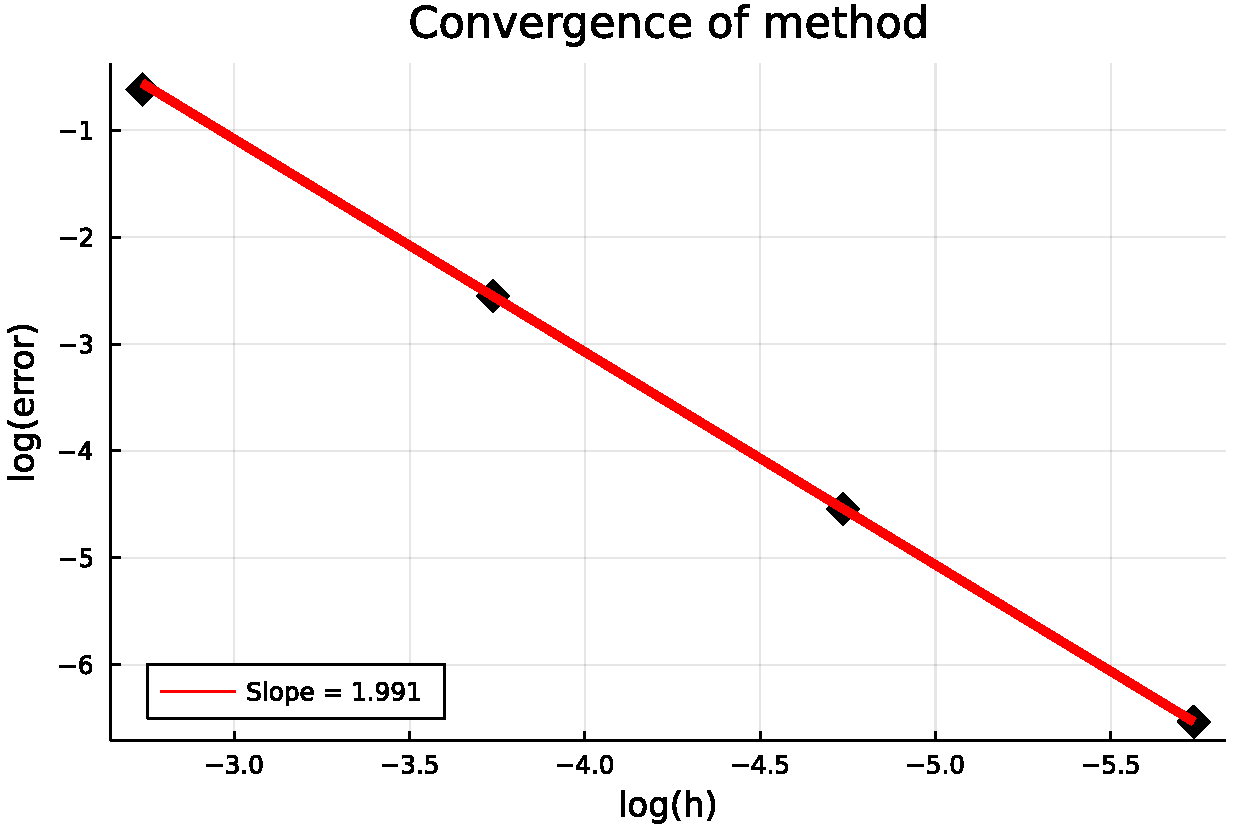
\includegraphics[width=\linewidth]{convergence_helmholtz.pdf}
    \caption{Convergence plot of helmholtz problem on rectangle. The slope is determined by linear least squares, excluding the first point.}
    \label{fig:helmholtz_conv}
\end{figure}

\subsection{Frequency response}
Now I apply the method on a more complex domain to study the depence on the wavenumber k.

\subsubsection{Mesh}
The mesh I use is shown in Figure \ref{fig:mesh}.
\begin{figure}
    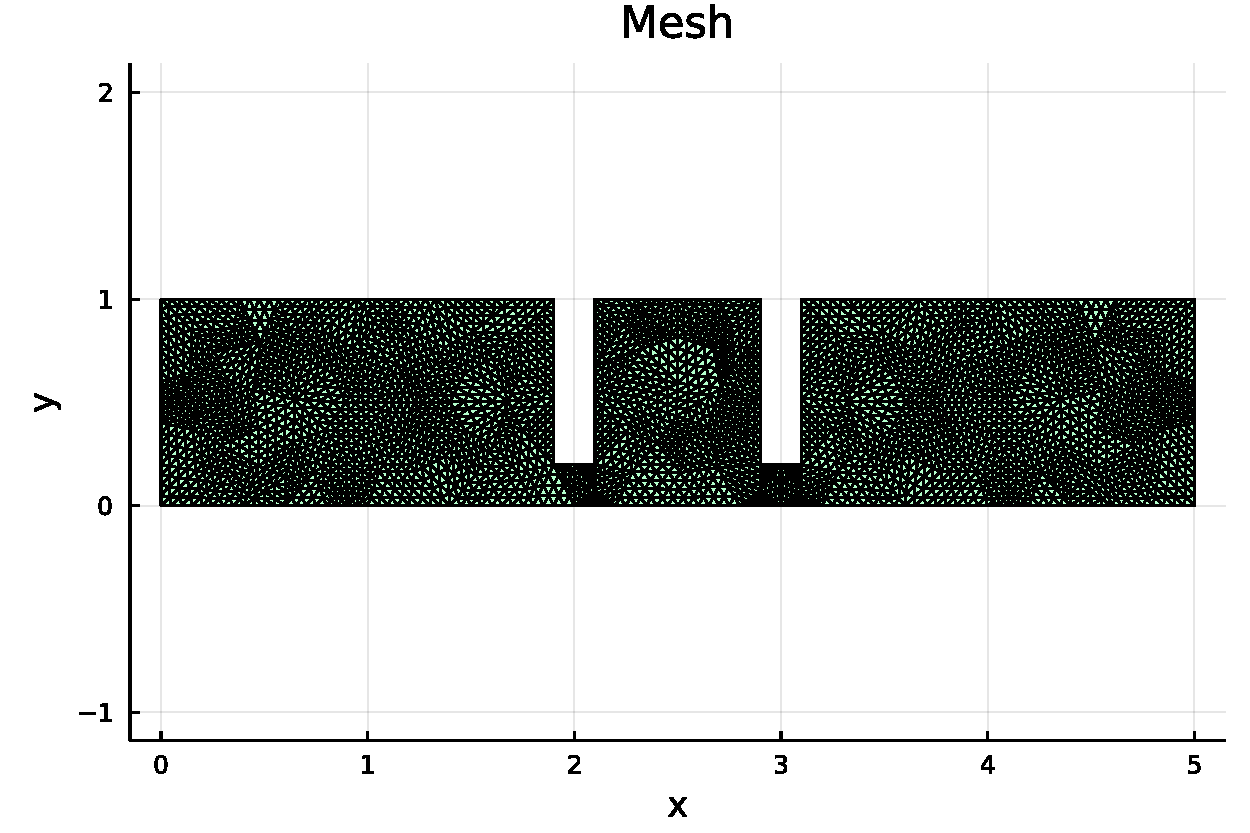
\includegraphics[width=\linewidth]{mesh.pdf}
    \caption{Mesh with double slit}
    \label{fig:mesh}
\end{figure}

\subsubsection{Intensity and wavenumber}
For a range of wavenumbers $k$ between $k=6$ and $6.5$, I plot the intensity. This is shown in the top figure of Figure \ref{fig:HvK}. The intensity is quite high in the lower range of wavenumbers, then gradually falling, until reaching a bottom around $k=6.35$, before rising again, though not to the same level as before, then finally decresing again at the end of the range of wavenumbers.

\begin{figure}
    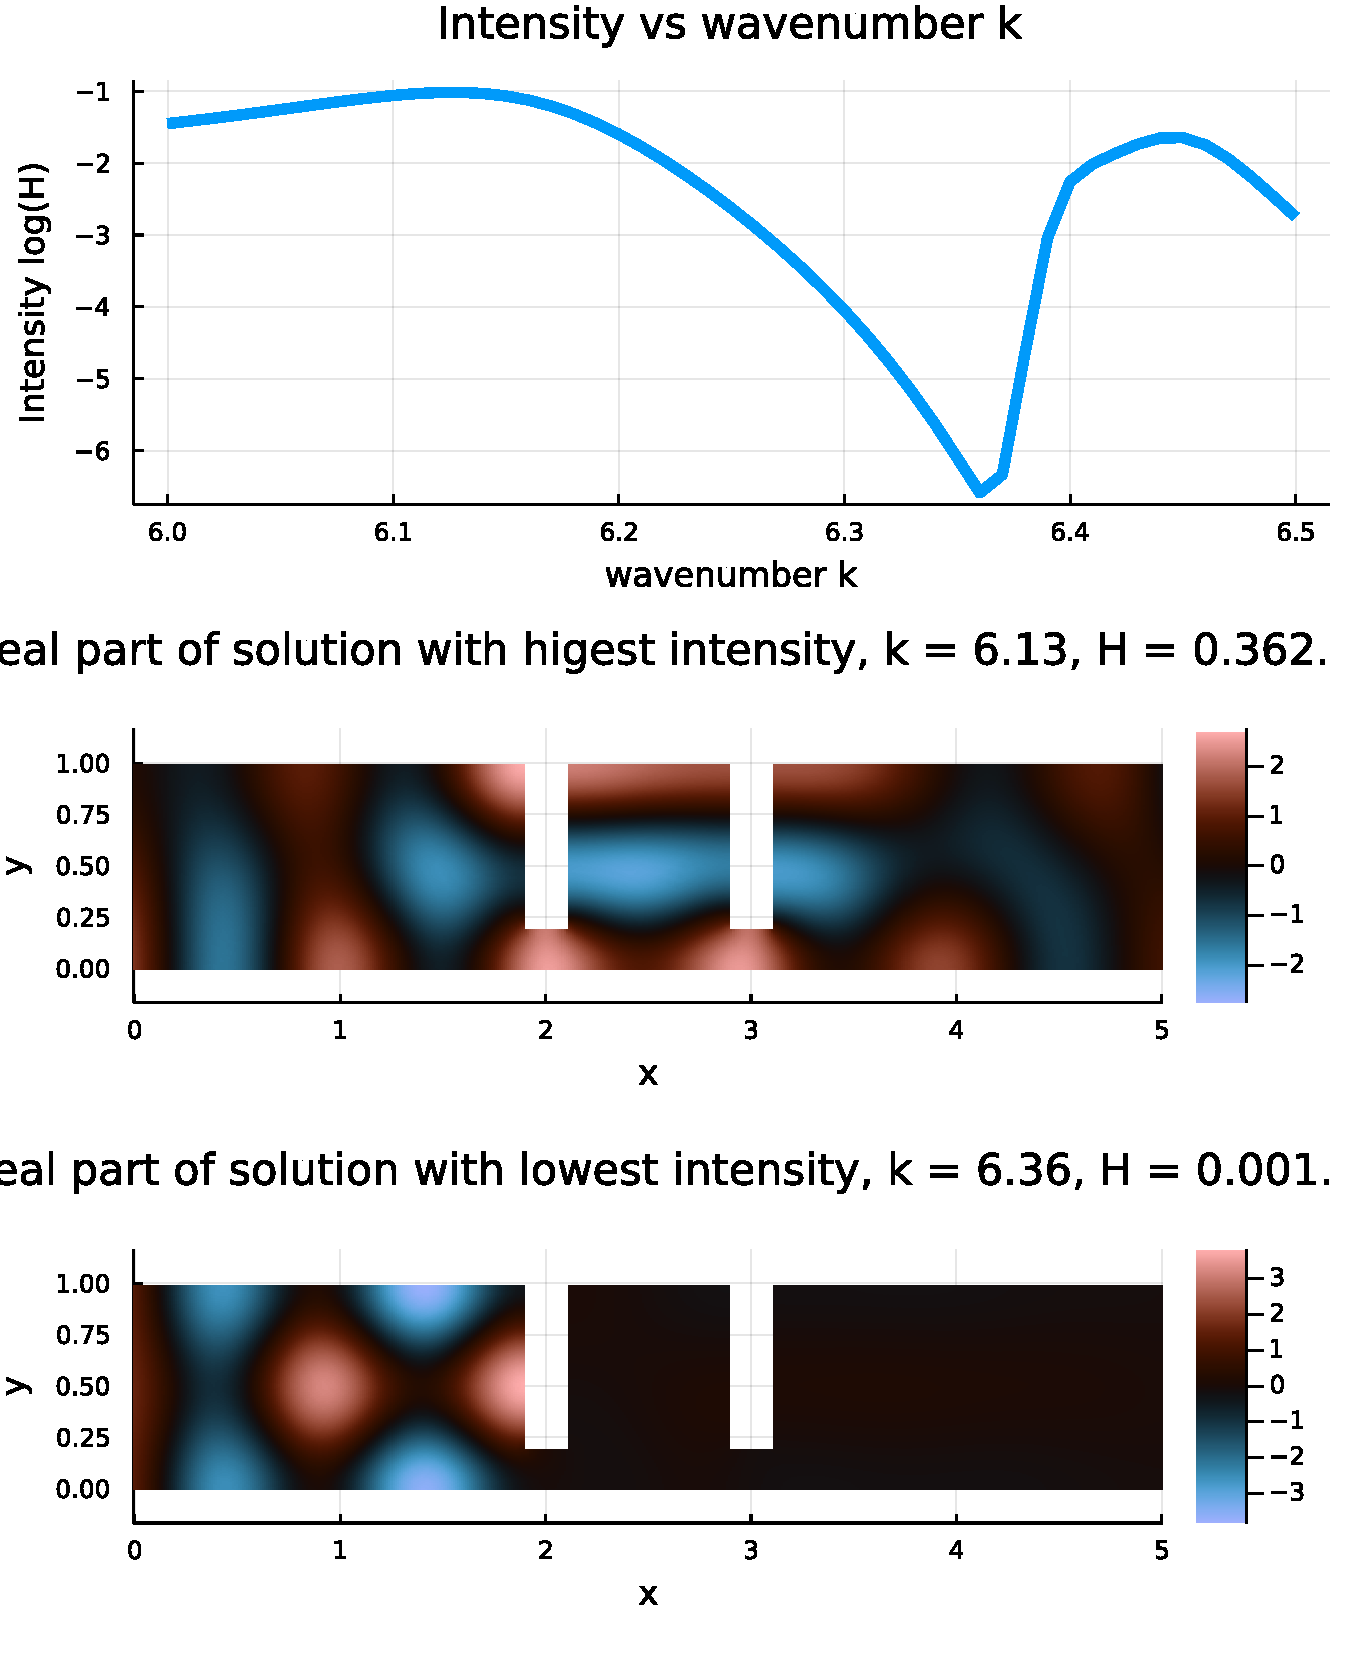
\includegraphics[width=\linewidth]{IvK_mx_mn.pdf}
    \caption{\textbf{Top}: Intensity as function of wavenumber.\textbf{Middle}: Solution corresponding to highest intensity \textbf{Bottom}: Solution corresponding to lowest intensity}
    \label{fig:HvK}
\end{figure}

\subsubsection{Highest and lowest intensity}
In the middle and bottom figure in Figure \ref{fig:HvK}, I show the solution corresponding to highest and lowest intensity, with $k=6.13$ and $k=6.36$, respectively. For the highest intensity, it seems like a lot of the energy of the wave is trapped in the central chambre, while for the lowest instenisty, almost nothing of the wave makes it into this cambre in the first place.

\newpage
\section*{Quadratic element for Poisson's equation}
I will here again solve Poisson's equation, $-\nabla^2 u=1$, with Dirichlet bounary conditions on the entire boundary, on a unit square, using quadratic elements instead of linear.

\subsection{Quadratic mesh}
In order for the elements to be quadratic, the triangulation needs to have 6 points per triangle. In order for the basis functions to be continuos on the element boundaries, the 3 extra points are inserted as the midpoint on each edge. This also keeps the number of new points to a minimum, be letting them be shared between to elements then not on the bounadry. I write a function
\begin{verbatim}
    p2, t2, e2 = p2mesh(p, t)
\end{verbatim}
which inserts these new points and includes them in the triangulation $t$.

\subsection{Computing the matrix}
The quadratic basis functons are parameterized as
\begin{equation*}
    p_i(x,y)=a_i+b_ix+c_iy+d_ix^2+e_iy^2+f_ixy,
\end{equation*}
and the coefficients are found by inverting the vandermonde-matrix
\begin{equation*}
    \begin{pmatrix}
        a_1 & a_2 & a_3 & a_4 & a_5 & a_6 \\
        b_1 & b_2 & b_3 & b_4 & b_5 & b_6 \\
        c_1 & c_2 & c_3 & c_4 & c_5 & c_6 \\
        d_1 & d_2 & d_3 & d_4 & d_5 & d_6 \\
        e_1 & e_2 & e_3 & e_4 & e_5 & e_6 \\
        f_1 & f_2 & f_3 & f_4 & f_5 & f_6 \\
    \end{pmatrix} = \begin{pmatrix}
        x_1^0y_1^0 & x_1^1y_1^0 & x_1^0y_1^1 & x_1^2y_1^0 & x_1^0y_1^2 & x_1^1y_1^1 \\
        x_2^0y_2^0 & x_2^1y_2^0 & x_2^0y_2^1 & x_2^2y_2^0 & x_2^0y_2^2 & x_2^1y_2^1 \\
        x_3^0y_3^0 & x_3^1y_3^0 & x_3^0y_3^1 & x_3^2y_3^0 & x_3^0y_3^2 & x_3^1y_3^1 \\
        x_4^0y_4^0 & x_4^1y_4^0 & x_4^0y_4^1 & x_4^2y_4^0 & x_4^0y_4^2 & x_4^1y_4^1 \\
        x_5^0y_5^0 & x_5^1y_5^0 & x_5^0y_5^1 & x_5^2y_5^0 & x_5^0y_5^2 & x_5^1y_5^1 \\
        x_6^0y_6^0 & x_6^1y_6^0 & x_6^0y_6^1 & x_6^2y_6^0 & x_6^0y_6^2 & x_6^1y_6^1 \\
    \end{pmatrix}^{-1}
\end{equation*}

The element matrix $sA$ and load $sb$ has the entries
\begin{align*}
    sA_{ij} & = \int_{T_k}\nabla p_i \nabla p_jdx = \int_{T_k}\partial_xp_i\partial_xp_j+\partial_yp_i\partial_yp_jdx \\
    sb_i    & = \int_{T_k}p_idx.
\end{align*}

The integrals are evaluated using the second-order accurate numerical quadrature-rule given in the problem description. This is done and solution obtained by the function
\begin{verbatim}
    u = fempoi2(p2, t2, e2).
\end{verbatim}

\subsection{Convergence study}
On a square domain, I solve Poisson's equation with several different grades of mesh-refinement. The finest mesh is used as the true solution, and the error is computed as the max-norm of the difference between the solution and the true solution, evaluated at the points of the coarsest mesh. Figure \ref{fig:conv_fempoi2} shows the convergence of the method. The slope is 3,so the local error is of third-order, and the method is globally a second-order method.


\begin{figure}[b]
    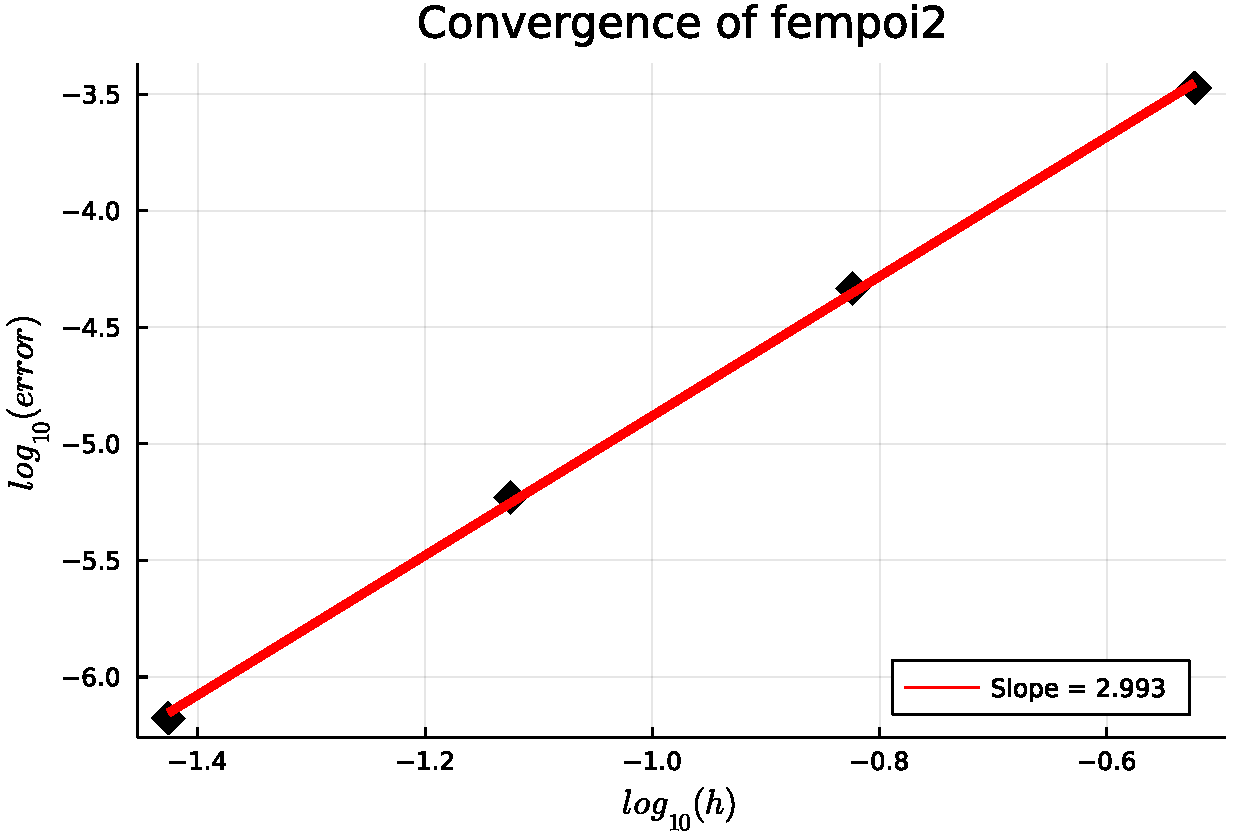
\includegraphics[width=\linewidth]{fempoi2_convergence.pdf}
    \caption{Convergence of finite element method with quadratic elements on Poisson's equation. The slope is determined by linear least squares, excluding the first point.}
    \label{fig:conv_fempoi2}
\end{figure}





\newpage
\appendix
\section{Element matrix of M} \label{apx:M}
I will here derive the element matrix for the matrix $M$, which is given as $M_{ij} = \int_{\Omega}\varphi_i\varphi_jdx$. To reduce indices, I let $\varphi_i=a+bx+cy$, and $\varphi_j=\alpha +\beta x + \gamma y$. Integrating a function $f(x, y)$ over a triangle $T_k$ with corners $(x_1, y_1), (x_2,y_2), (x_3,y_3)$ is done by transforming the triangle into the unit triangle $T_0$, giving the integral
\begin{align*}
    \iint_{T_k}f(x,y)dxdy & = |J|\int_0^1\int_0^{1-u}f(u, v)dvdu = |J|I,
    \\
    |J|                   & =\frac{\text{area}(T_k)}{\text{area}(T_0)},
    \\
    f(u, v)               & =f(x(u,v),y(u,v)),
    \\
    z(u, v)               & = z_1 + u\cdot(z_2-z_1)+v\cdot(z_3-z_1),
    \\
    f(x, y)               & = \varphi_i(x,y)\varphi_j(x,y)=(a+bx+cy)(\alpha+\beta x+\gamma y)
    \\
                          & = a\alpha+(a\beta+\alpha b)x+(a\gamma+\alpha x)y+(b\gamma+\beta c)xy+b\beta x^2+c\gamma y^2,
\end{align*}
where $z$ works as a stand-in for $x$ and $y$.

The following 6 integrals are the first building blocks in finding the final answer.
\begin{align*}
     & \int_0^1\int_0^{1-u}dvdu = \frac{1}{2}
     &                                            & \int_0^1\int_0^{1-u}uvdvdu = \frac{1}{24}
    \\
     & \int_0^1\int_0^{1-u}udvdu = \frac{1}{6}
     &                                            & \int_0^1\int_0^{1-u}vdvdu = \frac{1}{6}
    \\
     & \int_0^1\int_0^{1-u}u^2dvdu = \frac{1}{12}
     &                                            & \int_0^1\int_0^{1-u}v^2dvdu = \frac{1}{12}
\end{align*}

Building on this, the following 3 integrals will let me write up the final answer.

\begin{align*}
    \int_0^1\int_0^{1-u}zdvdu   & = \frac{z_1+z_2+z_3}{6} = \frac{1}{6},
    \\
    \int_0^1\int_0^{1-u}z^2dvdu & = \frac{z_1^2+z_2^2+z_3^2+z_1z_2+z_1z_3+z_2z_3}{12} = \frac{1}{12},
    \\
    \int_0^1\int_0^{1-u}xydvdu  & = \frac{x_1y_1+x_2y_2+x_3y_3}{12}+\frac{x_1y_2+x_2y_1+x_1y_3+x_3y_1+x_2y_3+x_3y_2}{24} = \frac{1}{24},
\end{align*}
where I have used the fact that I am using the unit triangle $T_0$, with $(x_1,y_1)=(0,0), (x_2,y_2)=(0,1), (x_3,y_3)=(1,0)$.
Combining it all, I get
\begin{equation*}
    I = \frac{a\alpha}{2}+\frac{a\beta+\beta a}{6}+\frac{a\gamma+\alpha x}{6} + \frac{b\beta}{12}+\frac{c\gamma}{12}+\frac{b\gamma+\beta c}{24}.
\end{equation*}
On $T_0$, the 3 basis function takes the form
\begin{equation*}
    \varphi_1 = 1-x-y, \hspace{4mm} \varphi_2=x, \hspace{4mm} \varphi_3=y.
\end{equation*}

Evauluating this, the final element matrix becomes
\begin{equation*}
    sM = 2\text{area}(T_k)\frac{1}{24}\begin{pmatrix}
        2 & 1 & 1 \\ 1 & 2 & 1 \\ 1 & 1 & 2
    \end{pmatrix}
\end{equation*}



\end{document}

